%\PassOptionsToPackage{table}{xcolor}
\documentclass{beamer}
\usepackage{amsmath, mathtools} % If amsmath is required
\usepackage{times,helvet,epsfig,color}
\usepackage{graphicx}
\usepackage{comment}
\usepackage{xspace}
\usepackage{hyperref}
%\PassOptionsToPackage{usenames}{xcolor}
\usepackage{overpic}
\graphicspath{{../img/}}
\mode<presentation>
{
	\usetheme{default} % I sometimes also use Warsaw
	\setbeamertemplate{itemize items}[circle]
	\setbeamertemplate{navigation symbols}{}
}
\setbeamertemplate{footline}
{
  \leavevmode%
  \hbox{%
  \begin{beamercolorbox}[wd=.3\paperwidth,ht=2.25ex,dp=1ex,left]{?}%
\hspace{1mm}
% \includegraphics[width=0.15\paperwidth]
%    {../../../current-docs/CarletonWide_K_186.png}
  \end{beamercolorbox}%
  \begin{beamercolorbox}[wd=.4\paperwidth,ht=2.25ex,dp=1ex,center]{title in head/foot}%
{\em 3D GREIT}, Grychtol, M\"uller, Adler, 2015/06/03
  \end{beamercolorbox}%
  \begin{beamercolorbox}[wd=.3\paperwidth,ht=2.25ex,dp=1ex,right]{title in head/foot}%
    \insertframenumber{}~/~\inserttotalframenumber\hspace*{1ex}
  \end{beamercolorbox}}%
  \vskip0pt%
}


\usepackage{tikz}
\pgfdeclarelayer{foreground}
 \pgfdeclarelayer{background}
 \pgfsetlayers{background,main,foreground}

\newcommand{\xB}{\mbox{$\mathbf{x}$}}
\newcommand{\xT}{\mbox{$\mathbf{\tilde x}$}}
\newcommand{\RB}{\mbox{$\mathbf{R}$}}
\newcommand{\yB}{\mbox{$\mathbf{y}$}}
\newcommand{\wB}{\mbox{$\mathbf{w}$}}

\begin{document}
\newcommand{\argmin}{\operatornamewithlimits{arg\,min}}
\DeclarePairedDelimiter{\norm}{\lVert}{\rVert}%


\title[3D GREIT]{
\vspace{10mm}
~\\
\Huge
{\em 3D Image Reconstruction with GREIT}
\\
\vspace{10mm}
}
\author{Bart\l{}omiej Grychtol$^1$,
Beat M\"uller$^2$, and
Andy Adler$^3$}
\institute[]{$^1$Fraunhofer Project Group for Automation in Medicine and 
Biotechnology, Mannheim, Germany 
\\
$^2$Swisstom AG, Landquart, Switzerland 
\\
$^3$Systems and Computer Engineering, Carleton University, Ottawa, Canada}
\date{}

\frame{\titlepage} 

\frame{\frametitle{%
Table of contents
}
\tableofcontents[currentsection]
}

\section{Motivation}
\frame{\frametitle{%
Motivation
}
\begin{itemize}
	\item[] Measurement setup already exists
	\begin{itemize}
		\item Swisstom Pioneer Set with 32 electrodes
		\item Watertank with 4 rings of connectors.
	\end{itemize}
	\item[]
	\item[] GREIT in EIDORS
	\begin{itemize}
		\item Forward model 3D
		\item Extension of image plane to 3D
	\end{itemize}
\end{itemize}
}

\section{GREIT}
\frame{\frametitle{%
GREIT
}
\begin{equation}
\RB = \argmin_{\footnotesize\RB}\sum_k \norm*{\xT^{(k)} - 
\RB\yB^{(k)}}^2_{\wB^{(k)}}
\end{equation}
\begin{itemize}
	\item $\RB$: Reconstruction matrix
	\item $k$ Training pairs $\{\xT^{(i)},\yB^{(i)}\}$
	\item $\xT^{(i)}$: Desired image of training disturbance $i$
	\item $\yB^{(i)}$: Voltages of training disturbance $i$
\end{itemize}
}

\frame{\frametitle{%
GREIT: Voltages of training disturbances
}
Solve forward problem:		
\begin{itemize}
	\item 3D FEM model 
	\item Placement of electrodes
\end{itemize}
Code available in EIDORS v3.8.
}

\frame{\frametitle{%
GREIT: Desired image
}
\begin{center}
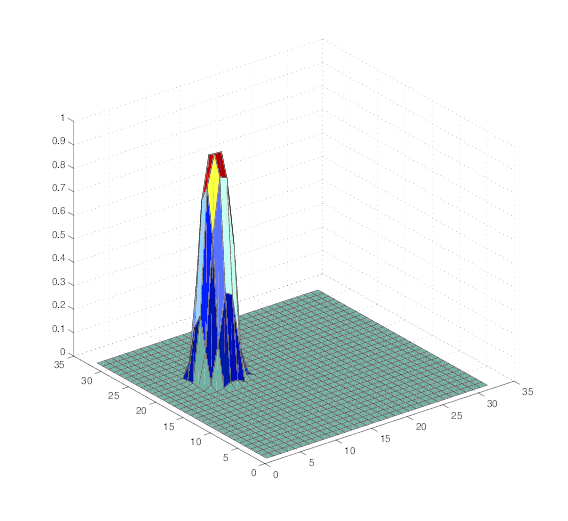
\includegraphics[width=.5\columnwidth]{desiredSolution.png}
\end{center}
Main enhancements needed in EIDORS.
\begin{itemize}
	\item Extend image plane from 2D to 3D
	\item Redefine desired image
\end{itemize}
}

\frame{\frametitle{%
GREIT: Training disturbances
}		
Some small extensions in EIDORS.
\begin{itemize}
	\item Distribution over whole object 
	\item What happens to off-plane objects?
\end{itemize}
Image plane may not cover whole FE model.
}

\frame{\frametitle{%
Reconstruction using real data
}
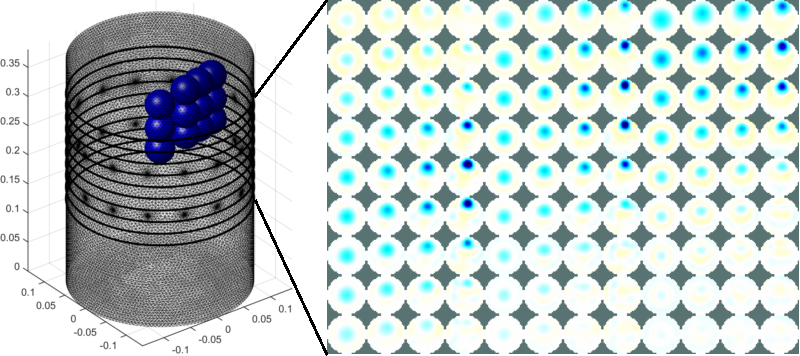
\includegraphics[width=\columnwidth]{tank_recon.pdf}
\\
\emph{Left:} FE model of a water tank with 
cut planes between voxel layers and positions of non-conductive 
target. \\
\emph{Right:} images reconstructed using the proposed algorithm. Each 
row corresponds to one voxel layer, and each column to a different target 
position.
}

\section{And now?}
\frame{\frametitle{%
And now?
}
Electrode placement:
\begin{itemize}
	\item How many rings of electrodes?
	\item How to place the electrodes?
	\item Which skip-pattern to use?
\end{itemize}
\vspace{1cm}
\input{elOrdering.latex}
}

\frame{\frametitle{%
Electrode placement
}
\begin{center}
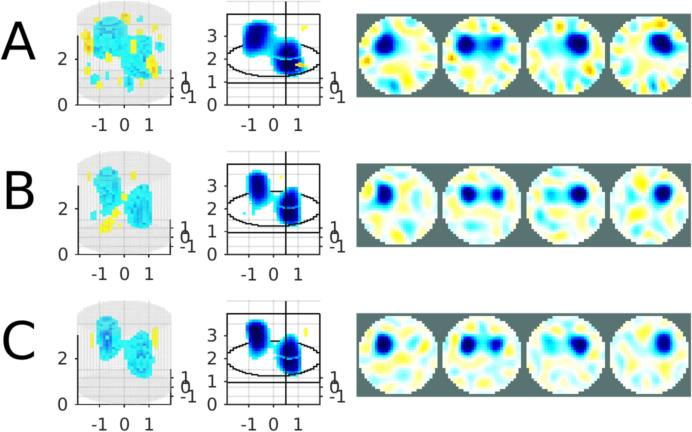
\includegraphics[width=0.7\columnwidth]{../img/greit-3d-example.jpg}
\end{center}
}

\frame{\frametitle{%
And now?
}
Visualization:
\begin{itemize}
	\item How to display the reconstructed images?
	\item[]
\end{itemize}

Figures of merit:
\begin{itemize}
	\item Do they still work?
	\item How to visualize them?
	\item[]
\end{itemize}

Off-plane objects:
\begin{itemize}
	\item How must off-plane objects taken into account? 
	\item[]
\end{itemize}
}


\section{Questions}
\frame{\frametitle{%
Any questions?
}
}

\end{document}

